\section{Design \& Implementation}
The system is created as a simple robot that can receive move instructions, and take measurements. The move instructions come from a PC running MATLAB. By receiving the measurement data the MATLAB application calculates the best movement action, and send it to the robot. 

The overall system design can be seen in figure \ref{fig:OSD}. The connection between the Computer and the Bluetooth shield is wireless. The connection between the Bluetooth shield and the Arduino Uno is serial. The connection between the Arduino Uno and LIDAR Sensor is serial and lastly the connection between the Arduino Robot and the Arduino Uno is i2c.
\begin{figure}[H]
\centering
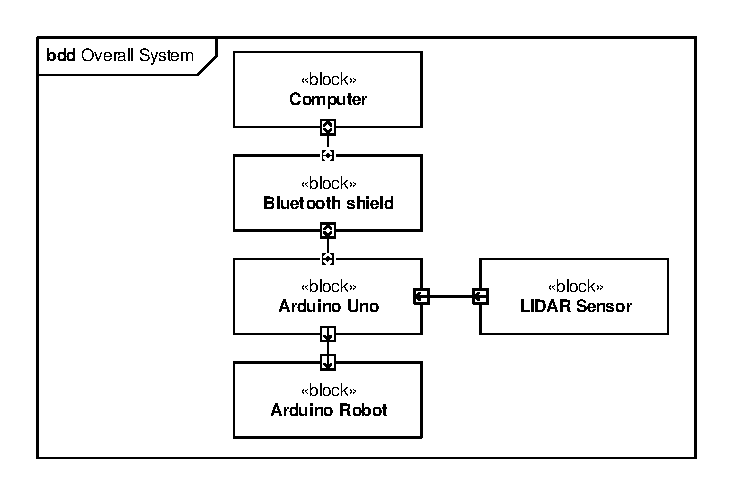
\includegraphics[width=0.7\textwidth]{billeder/OverallSystemDesign}
\caption{Overall System Design}
\label{fig:OSD}
\end{figure}
Each block in the system will now be discussed in greater detail. 

\subsubsection{Bluetooth shield}
The Bluetooth shield is an "ITEAD Wireless Bluetooth Shield Module Starter Kit For Arduino"\cite{BTshield}\cite{BTshield2}. The responsibility of the Bluetooth shield is to transfer data from the Arduino Uno to the Computer. The shield uses a HC-05 Serial Bluetooth module. Connecting to the shield is done by finding "H-C-2010-06-01" on the Computer and using the password: "1234". The settings for the serial bus is:
\begin{itemize}
\item Default baud rate: 9600
\item Data bits: 8
\item Stop bit: 1
\item No parity
\end{itemize}

This means that the Bluetooth connection can be seen as a simple uart connection between the robot and the computer. 

\subsubsection{LIDAR Sensor}
A LIDAR measurement consists of 90 packets with four range measurements in each. The packet length is 22 bytes and is organised as follows\cite{LIDAR}:
\begin{verbatim}
<start> <index> <speed_L> <speed_H> [Data 0] [Data 1] [Data 2] [Data 3]
 <checksum_L> <checksum_H>
\end{verbatim}
The $start$ code is 0xFA, $index$ goes from 0xA0 to 0xF9, $speed$ is the fixed point speed in RPM and $Data$ $N$ is the Nth reading. Each reading is four bytes in length and contains information about distance, signal strength and two flags. The data is comprised as follows:
\begin{verbatim}
<distance 7:0>  <"invalid data" flag> <"strength warning" flag> 
<distance 13:8> <signal strength 7:0> <signal strength 15:8>
\end{verbatim}
The LIDAR, also called Neato LIDAR can be seen in figure \ref{fig:NeatoLidar}.
\begin{figure}[H]
\centering
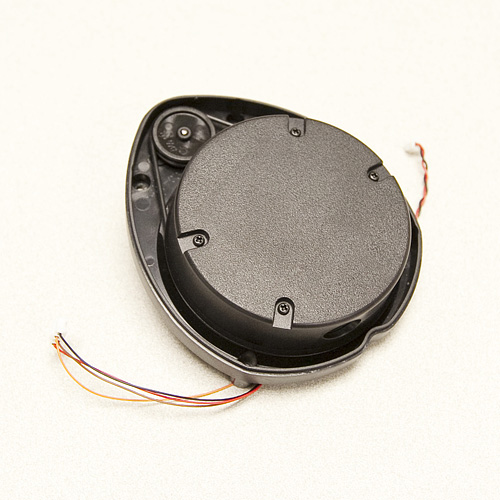
\includegraphics[scale=1]{billeder/NeatoLidar}
\caption{Neato LIDAR Sensor}
\label{fig:NeatoLidar}
\end{figure}
The LIDAR has four connects to the sensor part and two to the motor part. The motor connects are 3.3 Volt based with red being power and black being ground. The pinout for the sensor part is seen in table \ref{tab:lidars}.
\begin{table}[H]
\centering
\begin{tabular}{|l|l|}
\hline
Red & 3.3V \\ \hline
Brown & LDS\_RX \\ \hline
Orange & LDS\_TX \\ \hline
Black & GND \\ \hline
\end{tabular}
\caption{LIDAR Sensor Pinout}
\label{tab:lidars}
\end{table}

The motor is a simple DC-motor. But for a correct operation the Neato LIDAR must spin with more than 180 RPM and less than 350 RPM. The group found that a spin speed around 310 RPM gave the optimal sensor readings. This can be regulated using the speed information in the LIDAR data packets. The value in the speed bytes is formatted as RPM*64. So in order to get the RPM one must simply divide the value by 64. The group attained the optimal rotation speed, by regulating a PWM signal, on the motor. 

\subsubsection{Arduino Uno}
The Arduino Uno\cite{ArduinoUno} handles communication with the LIDAR Sensor and the Bluetooth shield.

\begin{figure}[H]
\centering
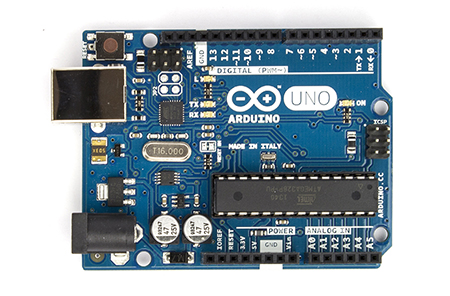
\includegraphics[scale=1]{billeder/ArduinoUno}
\caption{Arduino Uno}
\label{fig:ArduinoUno}
\end{figure}

The LIDAR data is streamed to the Arduino Uno contentiously with a baud rate on 115200. Therefore is the only hardware UART used to handle this. The data is stored in a internal array for later retrieval.

Since there is only one hardware UART on the Arduino Uno, and both the LIDAR and the bluetooth shield needs one, a software serial port is created to handle the bluetooth communication. 

The Arduino Uno is listening for commands, on the bluetooth connection. A command is formatted as follows: 
\begin{verbatim}
		<command ID 1> <command ID 2> [Command parameters ] < 0x0A ('\n') >
\end{verbatim}

The following commands is handled by the Arduino Uno: 

\begin{tabbing}	
LID \= AR:\\
\>{Command1: [LD D/S/P/E]} \\

\end{tabbing}	

  

\subsubsection{Arduino Robot}
The robot platform used in this project is a Arduino robot\cite{ArduinoRobot}. The Arduino robot platform handles all movement commands.

% Designandimp_Motion
\subsection{Motion}
The motion of the robot consists of two actions.
\begin{itemize}
\item Move forward 
\item Turn
\end{itemize}
Due to the lack of tachometers the robot needs an alternative way of figuring out how far it has moved or turned. The motion commands are therefore mainly based on time.

A general Move command is called by the command \textit{Move( socket, motor1, motor2, time )}, where socket is the bluetooth socket, motor1 is the speed of the right motor, motor2 is the speed of the left motor, both integer values in the range [-255:255], and time is the time in milliseconds.

\textbf{Move forward}\\
The Move forward command is called by the command \textit{[moved] = Move(obj, motor1, motor2, distance)}, where obj is the robot object, motor1 is the speed of the right motor, motor2 is the speed of the left motor, both integer values in the range [-255:255], and distance is the distance in cm. The moved parameter is the output of the Move forward command and contains the actual distance moved, based on LIDAR data.

This function consists of 2 parts. 
\begin{itemize}
\item Calculation of the time the robot must move to reach the desired distance.
\item Make sure that the robot does not bump into anything.
\end{itemize}
To find the time it takes for the robot to move, a measurement was made. The robot was placed behind a line, and different times were given to the function. The distance the robot travelled was then measured. In the end a function was fitted to the curve, and this function is the basic of the Move function.

\begin{figure}[H]
\centering
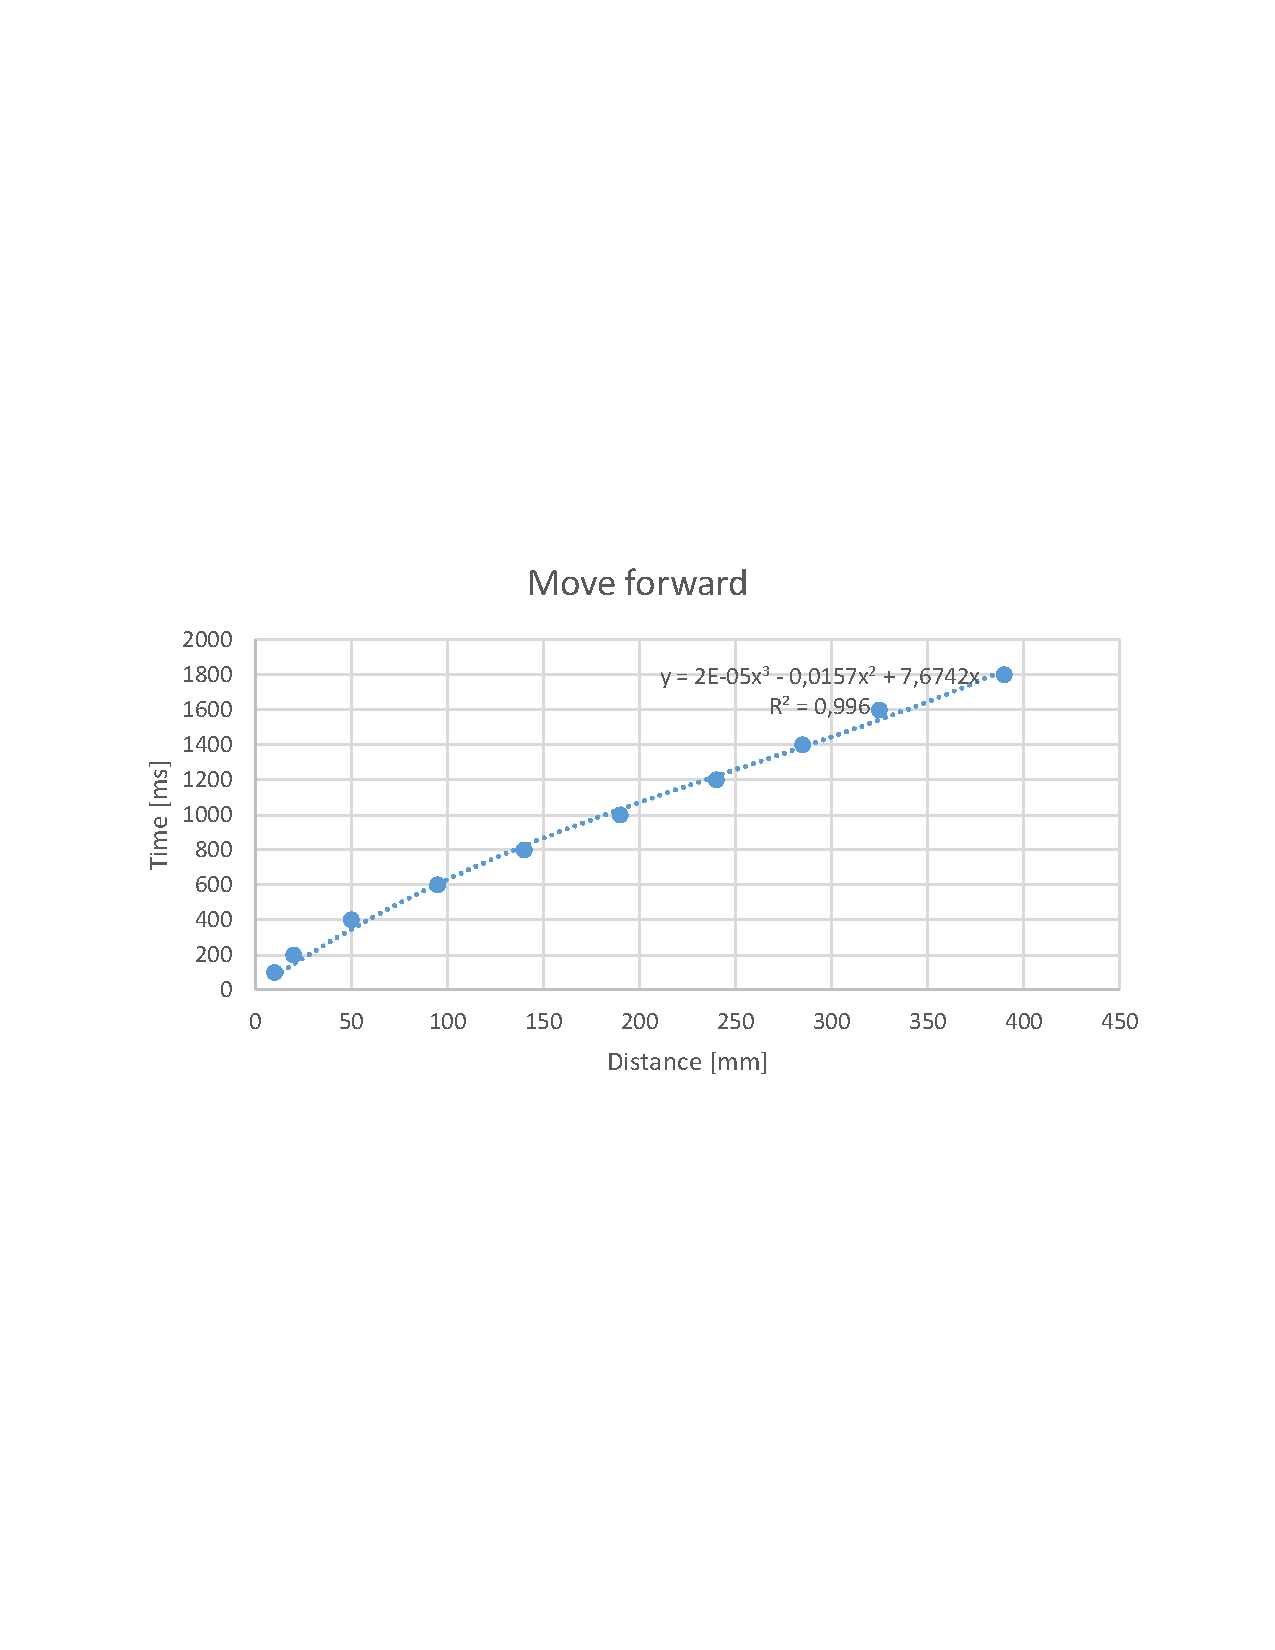
\includegraphics[width=0.8\textwidth]{billeder/MoveForwardGraph.pdf}
\caption{Measurement of Move forward}\label{MoveForwardGraph}
\end{figure} 

The main problem is that when the robot is using up battery, it does not move as far in the same given time as when it is fully charged. Therefore a measurement is made with the LIDAR before and after the movement to get a better fit of how far the robot actually moved. The measurement takes account of failing measurements, so that if the measurement straight ahead fails, it will use the nearest angle instead. The two distances is then calculated using trigonometry.
The difference between the two distances is the actual movement of the robot, and it is this value that is returned from the function.
The reason why LIDAR is not used directly to move a specific distance is the update rate of the LIDAR data. It is simply too slow. The function then calls the general Move command with the calculated time.

Despite the fact that the LIDAR has a slow update rate, it is used as a safe distance detection. If an object is detected in the area shown in figure \ref{MotionBumper}, the robot stops its movement and the function returns the moved distance. Due to the slow update rate of the LIDAR, the safe distance is relatively high. In the project, the forward safety distance is set to 250 mm. and the safety distance to each side is 200 mm.

\begin{figure}[H]
\centering
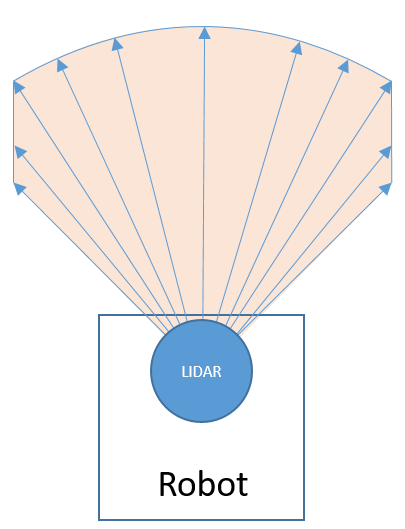
\includegraphics[scale=0.7]{billeder/MotionBumper.png}
\caption{Area of bump detection. The robot is facing up.}\label{MotionBumper}
\end{figure} 

\textbf{Turn}\\
The Turn command is called by the command \textit{Turn(obj, phi)}, where obj is the robot object and phi is the turning angle in degrees. The range of phi is [-180:180] with decimals accepted. This function calculates the time it will take for the robot to turn to the angle received, and calls the general Move function with one motor in reverse and the other in forward position. 
To get a way to calculate the time, a measurement similar to the on for the Move forward function was made. The robot was placed at a point and a mark was made where it had its 0 degrees. Then the general move function was called with different times and the angle the robot turned was measured. Figure \ref{TurnRightGraph} and \ref{TurnLeftGraph} shows the result of the measurements.

\begin{figure}[H]
\centering
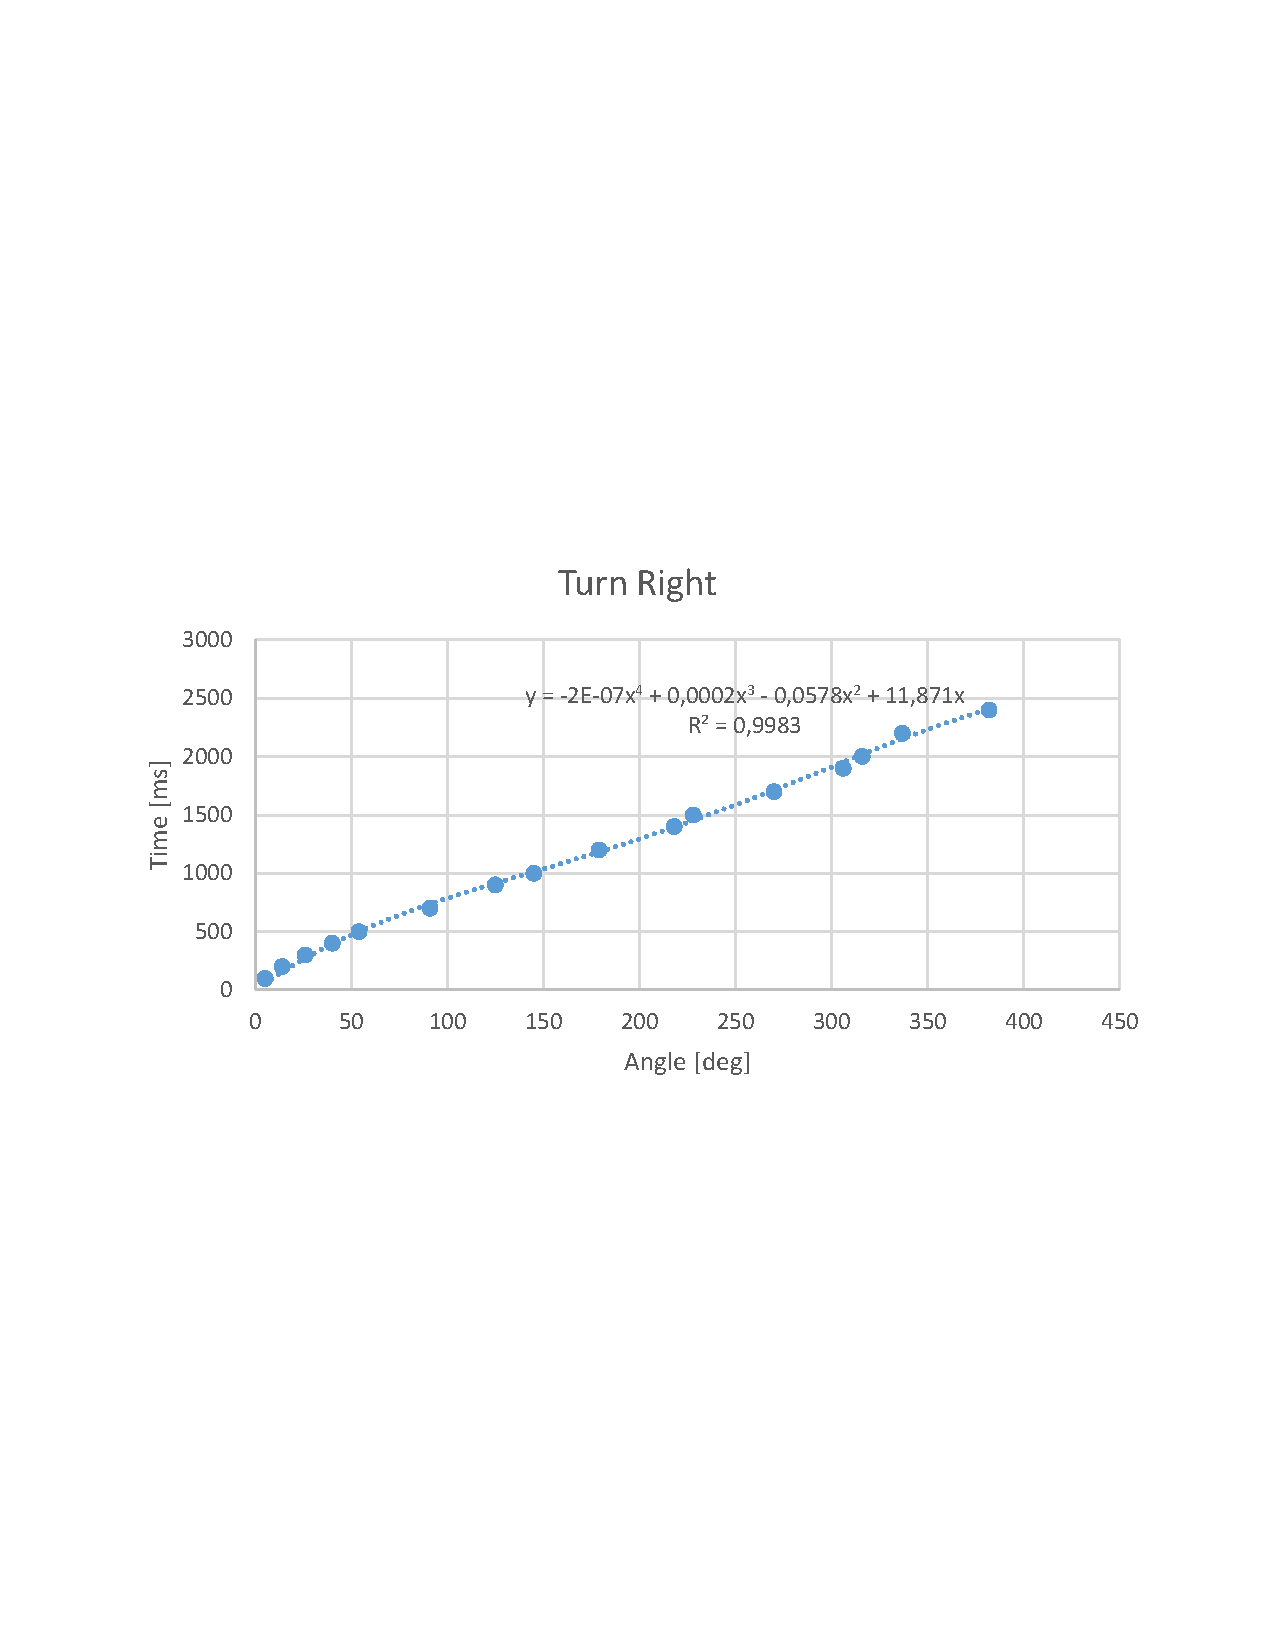
\includegraphics[width=0.8\textwidth]{billeder/TurnRightGraph.pdf}
\caption{Measurement of Turn right}\label{TurnRightGraph}
\end{figure} 
\begin{figure}[H]
\centering
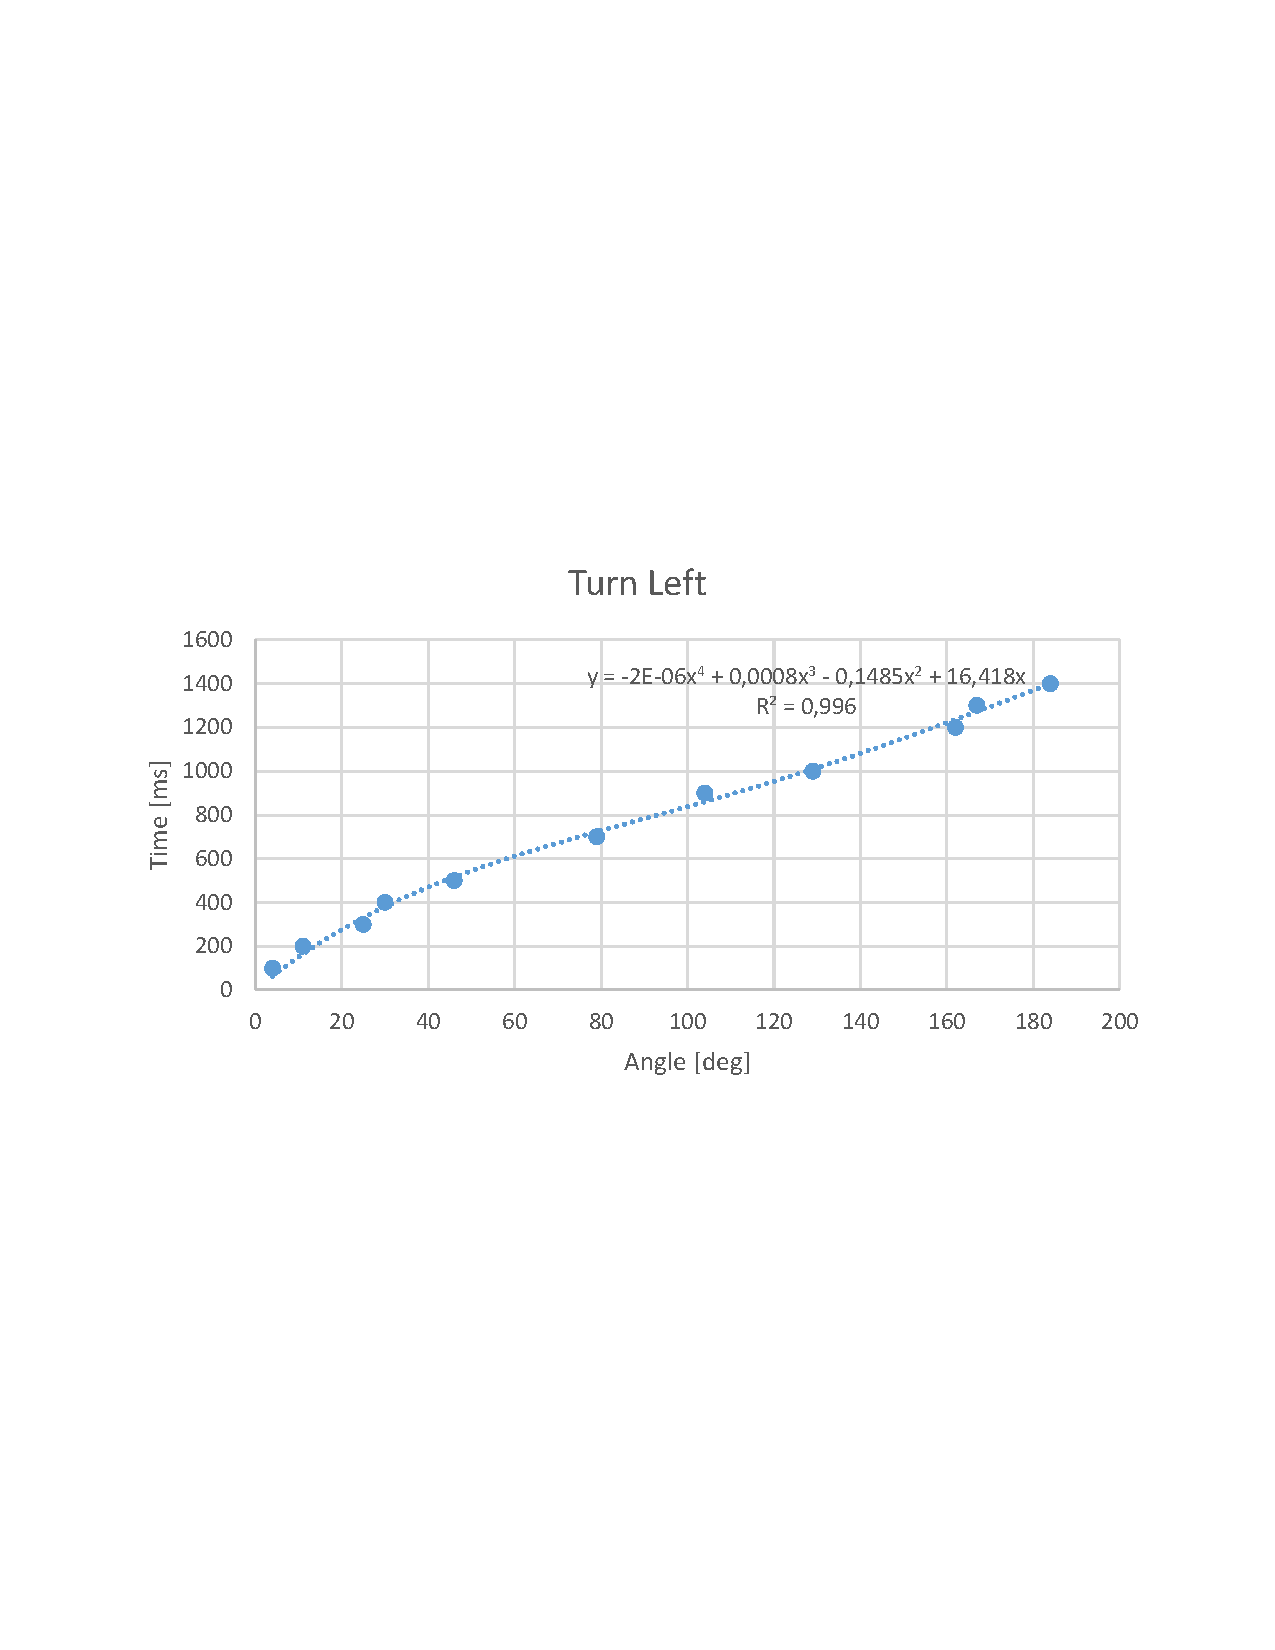
\includegraphics[width=0.8\textwidth]{billeder/TurnLeftGraph.pdf}
\caption{Measurement of Turn left}\label{TurnLeftGraph}
\end{figure} 

The same problem with the battery power arises in this function. Therefore a scanning is made by the LIDAR before the turn is performed. After the turn is made, the LIDAR scans again and the robot compares the two measurements by convolution. Then it starts to step one degree until a maximum in the convolution is found. This is then expected to be a more correct guess of the desired angle.

 
%------------------------------------------------